\documentclass[8pt,aspectratio=169]{beamer}
\usetheme{Madrid}
\usepackage{graphicx,booktabs,adjustbox,multicol,amsmath,amssymb,listings,xcolor,colortbl}
\definecolor{mlblue}{RGB}{0,102,204}
\definecolor{mlpurple}{RGB}{51,51,178}
\definecolor{mllavender}{RGB}{173,173,224}
\definecolor{mllavender2}{RGB}{193,193,232}
\definecolor{mllavender3}{RGB}{204,204,235}
\definecolor{mllavender4}{RGB}{214,214,239}
\definecolor{mlorange}{RGB}{255,127,14}
\definecolor{mlgreen}{RGB}{44,160,44}
\definecolor{mlred}{RGB}{214,39,40}
\definecolor{mlgray}{RGB}{127,127,127}
% Solidity colors
\definecolor{solkeyword}{RGB}{0,102,153}
\definecolor{solstring}{RGB}{163,21,21}
\definecolor{solcomment}{RGB}{0,128,0}
\definecolor{solnumber}{RGB}{0,128,128}
\setbeamercolor{palette primary}{bg=mllavender3,fg=mlpurple}
\setbeamercolor{palette secondary}{bg=mllavender2,fg=mlpurple}
\setbeamercolor{palette tertiary}{bg=mllavender,fg=white}
\setbeamercolor{palette quaternary}{bg=mlpurple,fg=white}
\setbeamercolor{structure}{fg=mlpurple}
\setbeamercolor{title}{fg=mlpurple}
\setbeamercolor{frametitle}{fg=mlpurple,bg=mllavender3}
\setbeamercolor{block title}{bg=mllavender2,fg=mlpurple}
\setbeamercolor{block body}{bg=mllavender4,fg=black}
\setbeamertemplate{navigation symbols}{}
\setbeamertemplate{itemize items}[circle]
\setbeamersize{text margin left=5mm,text margin right=5mm}
\newcommand{\bottomnote}[1]{\vfill\vspace{-2mm}\textcolor{mllavender2}{\rule{\textwidth}{0.4pt}}\par\vspace{1mm}{\footnotesize\textbf{\adjustbox{max width=\textwidth}{#1}}}}
% Solidity language definition
\lstdefinelanguage{Solidity}{
  keywords={pragma, solidity, contract, function, public, private, external, internal, view, pure, payable, returns, return, if, else, for, while, mapping, address, uint, uint256, int, string, bool, bytes, bytes32, event, emit, modifier, require, constructor, memory, storage, calldata, msg, sender, value, this, new, delete, true, false, import, is, constant, override, virtual},
  keywordstyle=\color{solkeyword}\bfseries,
  sensitive=true,
  comment=[l]{//},
  morecomment=[s]{/*}{*/},
  commentstyle=\color{solcomment}\ttfamily,
  stringstyle=\color{solstring}\ttfamily,
  morestring=[b]',
  morestring=[b]"
}
\lstset{language=Solidity,basicstyle=\ttfamily\scriptsize,breaklines=true,frame=single,backgroundcolor=\color{mllavender4},numbers=left,numberstyle=\tiny\color{mlgray},numbersep=5pt,tabsize=2,showstringspaces=false}
\usepackage{tikz}
\usetikzlibrary{arrows.meta,positioning,shapes.geometric,calc,chains,decorations.pathmorphing,automata,fit}
\usepackage{pgfplots}
\pgfplotsset{compat=1.18}
\title{Deploy Your First Crypto Token --- A Visual Recipe}
\subtitle{Standalone Beginner Walkthrough}
\author{Prof.~Dr.~Joerg Osterrieder}
\institute{University Lecture Series}
\date{\today}
\begin{document}

%% ============================================================
%% FRAME 1: TITLE PAGE
%% ============================================================
\begin{frame}[plain]
\vspace{2cm}
\begin{center}
{\Large\bfseries\color{mlpurple} Deploy Your First Crypto Token}\\[4mm]
{\large\color{mlblue} A Visual Recipe}\\[8mm]
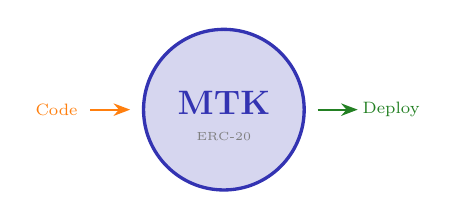
\begin{tikzpicture}[scale=0.85, every node/.style={transform shape}]
% Token icon
\draw[mlpurple, very thick, fill=mllavender4] (0,0) circle (1.2);
\node[font=\Large\bfseries, mlpurple] at (0,0.1) {MTK};
\node[font=\tiny, mlgray] at (0,-0.4) {ERC-20};
% Decorative arrows
\draw[-{Stealth[length=6pt]}, mlorange, thick] (-2.0,0) -- (-1.4,0);
\draw[-{Stealth[length=6pt]}, mlgreen!80!black, thick] (1.4,0) -- (2.0,0);
\node[font=\scriptsize, mlorange] at (-2.5,0) {Code};
\node[font=\scriptsize, mlgreen!80!black] at (2.5,0) {Deploy};
\end{tikzpicture}
\\[6mm]
{\footnotesize Prof.~Dr.~Joerg Osterrieder}\\[1mm]
{\footnotesize\color{mlgray} University Lecture Series}
\end{center}
\end{frame}

%% ============================================================
%% FRAME 2: WHAT YOU'LL NEED (4-icon TikZ grid)
%% ============================================================
\begin{frame}{What You'll Need}
\begin{center}
\adjustbox{max width=\textwidth}{%
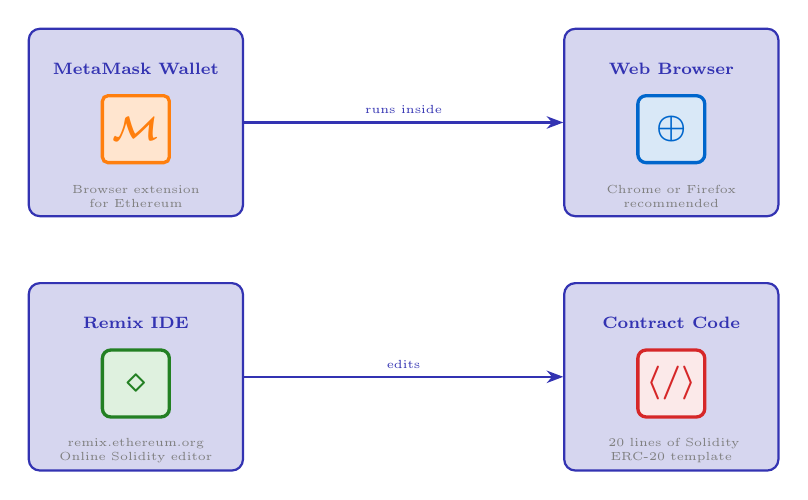
\begin{tikzpicture}[scale=0.85, every node/.style={transform shape},
  iconbox/.style={draw=mlpurple, thick, fill=mllavender4, rounded corners=4pt,
    minimum width=3.2cm, minimum height=2.8cm, align=center}]

% Row 1
\node[iconbox] (mm) at (-4,1.8) {};
\node[font=\scriptsize\bfseries, mlpurple] at (-4,2.6) {MetaMask Wallet};
% Fox icon (simplified)
\draw[mlorange, very thick, fill=mlorange!20, rounded corners=2pt] (-4.5,1.2) rectangle (-3.5,2.2);
\node[font=\Large, mlorange] at (-4,1.7) {$\boldsymbol{\mathcal{M}}$};
\node[font=\tiny, mlgray, text width=2.8cm, align=center] at (-4,0.7) {Browser extension\\for Ethereum};

\node[iconbox] (br) at (4,1.8) {};
\node[font=\scriptsize\bfseries, mlpurple] at (4,2.6) {Web Browser};
\draw[mlblue, very thick, fill=mlblue!15, rounded corners=3pt] (3.5,1.2) rectangle (4.5,2.2);
\node[font=\Large, mlblue] at (4,1.7) {$\boldsymbol{\oplus}$};
\node[font=\tiny, mlgray, text width=2.8cm, align=center] at (4,0.7) {Chrome or Firefox\\recommended};

% Row 2
\node[iconbox] (rx) at (-4,-2.0) {};
\node[font=\scriptsize\bfseries, mlpurple] at (-4,-1.2) {Remix IDE};
\draw[mlgreen!80!black, very thick, fill=mlgreen!15, rounded corners=3pt] (-4.5,-2.6) rectangle (-3.5,-1.6);
\node[font=\Large, mlgreen!80!black] at (-4,-2.1) {$\boldsymbol{\diamond}$};
\node[font=\tiny, mlgray, text width=2.8cm, align=center] at (-4,-3.1) {remix.ethereum.org\\Online Solidity editor};

\node[iconbox] (cc) at (4,-2.0) {};
\node[font=\scriptsize\bfseries, mlpurple] at (4,-1.2) {Contract Code};
\draw[mlred, very thick, fill=mlred!10, rounded corners=3pt] (3.5,-2.6) rectangle (4.5,-1.6);
\node[font=\Large, mlred] at (4,-2.1) {$\boldsymbol{\langle/\rangle}$};
\node[font=\tiny, mlgray, text width=2.8cm, align=center] at (4,-3.1) {~20 lines of Solidity\\ERC-20 template};

% Connecting arrows
\draw[-{Stealth[length=6pt]}, mlpurple, thick] (mm.east) -- (br.west)
  node[midway, above, font=\tiny] {runs inside};
\draw[-{Stealth[length=6pt]}, mlpurple, thick] (rx.east) -- (cc.west)
  node[midway, above, font=\tiny] {edits};

\end{tikzpicture}%
}%
\end{center}

\bottomnote{All tools are free --- MetaMask is a browser extension, Remix is a web app, and testnet ETH costs nothing.}
\end{frame}

%% ============================================================
%% FRAME 3: THE MISSION (Comic Strip - 3 panels)
%% ============================================================
\begin{frame}{The Mission}
\begin{center}
\adjustbox{max width=\textwidth}{%
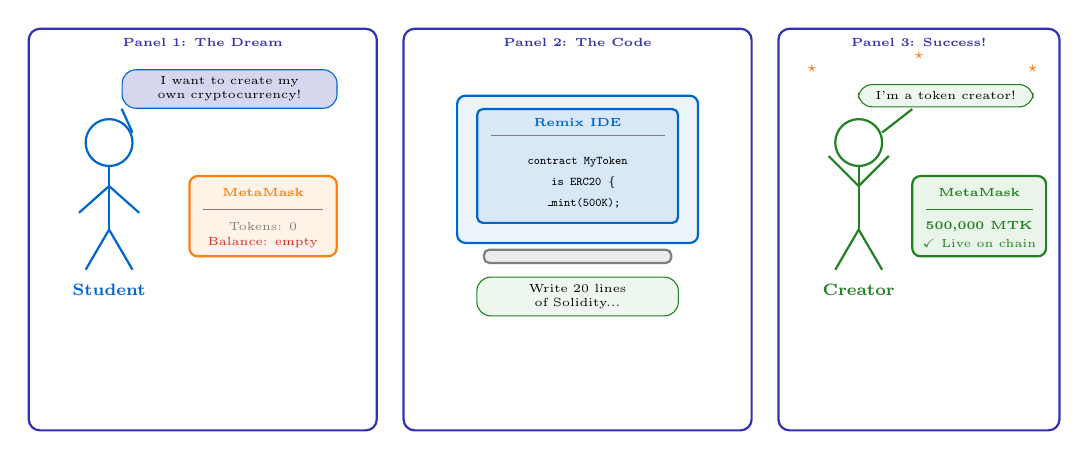
\begin{tikzpicture}[scale=0.85, every node/.style={transform shape}]

% --- Panel 1: Student with empty wallet ---
\draw[mlpurple, thick, rounded corners=4pt] (-7.2,-2.8) rectangle (-2.0,3.2);
\node[font=\tiny\bfseries, mlpurple] at (-4.6,3.0) {Panel 1: The Dream};

% Student stick figure
\draw[mlblue, thick] (-6.0,1.5) circle (0.35);
\draw[mlblue, thick] (-6.0,1.15) -- (-6.0,0.2);
\draw[mlblue, thick] (-6.0,0.85) -- (-6.45,0.45);
\draw[mlblue, thick] (-6.0,0.85) -- (-5.55,0.45);
\draw[mlblue, thick] (-6.0,0.2) -- (-6.35,-0.4);
\draw[mlblue, thick] (-6.0,0.2) -- (-5.65,-0.4);
\node[font=\scriptsize\bfseries, mlblue] at (-6.0,-0.7) {Student};

% MetaMask wallet box
\draw[mlorange, thick, fill=mlorange!10, rounded corners=3pt] (-4.8,-0.2) rectangle (-2.6,1.0);
\node[font=\tiny\bfseries, mlorange] at (-3.7,0.75) {MetaMask};
\draw[mlgray, thin] (-4.6,0.5) -- (-2.8,0.5);
\node[font=\tiny, mlgray] at (-3.7,0.25) {Tokens: 0};
\node[font=\tiny, mlred] at (-3.7,0.0) {Balance: empty};

% Speech bubble
\node[draw=mlblue, fill=mllavender4, rounded corners=5pt, font=\tiny,
      text width=3.0cm, align=center, inner sep=3pt]
      (stud-bubble) at (-4.2,2.3) {I want to create my own cryptocurrency!};
\draw[mlblue, thick] (-5.65,1.65) -- (stud-bubble.south west);

% --- Panel 2: Coding in Remix ---
\draw[mlpurple, thick, rounded corners=4pt] (-1.6,-2.8) rectangle (3.6,3.2);
\node[font=\tiny\bfseries, mlpurple] at (1.0,3.0) {Panel 2: The Code};

% Laptop / screen
\draw[mlblue, thick, fill=mlblue!8, rounded corners=3pt] (-0.8,0.0) rectangle (2.8,2.2);
\draw[mlblue, thick, fill=mlblue!15, rounded corners=2pt] (-0.5,0.3) rectangle (2.5,2.0);
\node[font=\tiny\bfseries, mlblue] at (1.0,1.8) {Remix IDE};
\draw[mlgray, thin] (-0.3,1.6) -- (2.3,1.6);
\node[font=\tiny, align=left] at (1.0,1.2) {\texttt{contract MyToken}};
\node[font=\tiny, align=left] at (1.0,0.9) {\texttt{~~is ERC20 \{}};
\node[font=\tiny, align=left] at (1.0,0.6) {\texttt{~~\_mint(500K);}};

% Speech bubble
\node[draw=mlgreen!80!black, fill=mlgreen!8, rounded corners=5pt, font=\tiny,
      text width=2.8cm, align=center, inner sep=3pt]
      at (1.0,-0.8) {Write 20 lines of Solidity...};

% Keyboard base
\draw[mlgray, thick, fill=mlgray!15, rounded corners=2pt] (-0.4,-0.3) rectangle (2.4,-0.1);

% --- Panel 3: Celebration ---
\draw[mlpurple, thick, rounded corners=4pt] (4.0,-2.8) rectangle (8.2,3.2);
\node[font=\tiny\bfseries, mlpurple] at (6.1,3.0) {Panel 3: Success!};

% Celebrating stick figure
\draw[mlgreen!80!black, thick] (5.2,1.5) circle (0.35);
\draw[mlgreen!80!black, thick] (5.2,1.15) -- (5.2,0.2);
\draw[mlgreen!80!black, thick] (5.2,0.85) -- (4.75,1.3);
\draw[mlgreen!80!black, thick] (5.2,0.85) -- (5.65,1.3);
\draw[mlgreen!80!black, thick] (5.2,0.2) -- (4.85,-0.4);
\draw[mlgreen!80!black, thick] (5.2,0.2) -- (5.55,-0.4);
\node[font=\scriptsize\bfseries, mlgreen!80!black] at (5.2,-0.7) {Creator};

% Wallet showing tokens
\draw[mlgreen!80!black, thick, fill=mlgreen!10, rounded corners=3pt] (6.0,-0.2) rectangle (8.0,1.0);
\node[font=\tiny\bfseries, mlgreen!80!black] at (7.0,0.75) {MetaMask};
\draw[mlgreen!80!black, thin] (6.2,0.5) -- (7.8,0.5);
\node[font=\tiny\bfseries, mlgreen!80!black] at (7.0,0.25) {500,000 MTK};
\node[font=\tiny, mlgreen!80!black] at (7.0,0.0) {$\checkmark$ Live on chain};

% Speech bubble
\node[draw=mlgreen!80!black, fill=mlgreen!8, rounded corners=5pt, font=\tiny,
      text width=2.4cm, align=center, inner sep=3pt]
      at (6.5,2.2) {I'm a token creator!};
\draw[mlgreen!80!black, thick] (5.55,1.65) -- (6.0,2.0);

% Celebration sparkles
\node[font=\scriptsize, mlorange] at (4.5,2.6) {$\star$};
\node[font=\scriptsize, mlorange] at (7.8,2.6) {$\star$};
\node[font=\scriptsize, mlorange] at (6.1,2.8) {$\star$};

\end{tikzpicture}%
}%
\end{center}

\bottomnote{Creating a token is writing a smart contract --- anyone can do it in minutes.}
\end{frame}

%% ============================================================
%% FRAME 4: STEP 1 - WRITE THE CONTRACT [fragile]
%% ============================================================
\begin{frame}[fragile]{Step 1 --- Write the Contract}
\vspace{-2mm}
\begin{columns}[T]
\begin{column}{0.58\linewidth}
\begin{lstlisting}[basicstyle=\ttfamily\tiny,xleftmargin=0pt,xrightmargin=0pt,linewidth=\linewidth]
// SPDX-License-Identifier: MIT
pragma solidity ^0.8.20;

import "@openzeppelin/contracts/token/ERC20/ERC20.sol";
import "@openzeppelin/contracts/access/Ownable.sol";

contract MyToken is ERC20, Ownable {
    uint256 public constant MAX_SUPPLY
        = 1_000_000 * 10**18;

    constructor()
        ERC20("MyToken", "MTK")
        Ownable(msg.sender)
    {
        _mint(msg.sender, 500_000 * 10**18);
    }

    function mint(address to, uint256 amount)
        public onlyOwner
    {
        require(
            totalSupply() + amount <= MAX_SUPPLY,
            "Exceeds cap"
        );
        _mint(to, amount);
    }

    function burn(uint256 amount) public {
        _burn(msg.sender, amount);
    }
}
\end{lstlisting}
\end{column}
\begin{column}{0.40\linewidth}
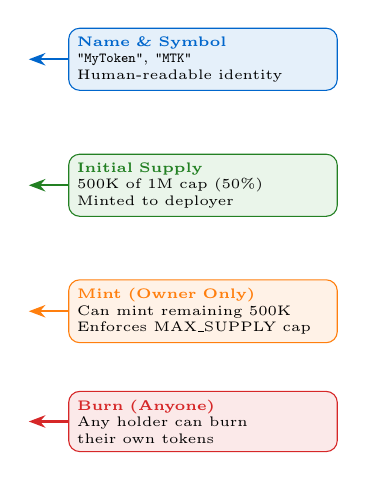
\begin{tikzpicture}[every node/.style={transform shape}]
% Blue callout - name/symbol
\node[draw=mlblue, fill=mlblue!10, rounded corners=4pt, font=\tiny,
      inner sep=3pt, text width=3.2cm, align=left]
      (c1) at (0,4.8) {\textbf{\color{mlblue}Name \& Symbol}\\
      \texttt{"MyToken"}, \texttt{"MTK"}\\
      Human-readable identity};
\draw[-{Stealth[length=6pt]}, mlblue, thick] (c1.west) -- ++(-0.5,0);

% Green callout - initial supply
\node[draw=mlgreen!80!black, fill=mlgreen!10, rounded corners=4pt, font=\tiny,
      inner sep=3pt, text width=3.2cm, align=left]
      (c2) at (0,3.2) {\textbf{\color{mlgreen!80!black}Initial Supply}\\
      500K of 1M cap (50\%)\\
      Minted to deployer};
\draw[-{Stealth[length=6pt]}, mlgreen!80!black, thick] (c2.west) -- ++(-0.5,0);

% Orange callout - mint
\node[draw=mlorange, fill=mlorange!10, rounded corners=4pt, font=\tiny,
      inner sep=3pt, text width=3.2cm, align=left]
      (c3) at (0,1.6) {\textbf{\color{mlorange}Mint (Owner Only)}\\
      Can mint remaining 500K\\
      Enforces MAX\_SUPPLY cap};
\draw[-{Stealth[length=6pt]}, mlorange, thick] (c3.west) -- ++(-0.5,0);

% Red callout - burn
\node[draw=mlred, fill=mlred!10, rounded corners=4pt, font=\tiny,
      inner sep=3pt, text width=3.2cm, align=left]
      (c4) at (0,0.2) {\textbf{\color{mlred}Burn (Anyone)}\\
      Any holder can burn\\
      their own tokens};
\draw[-{Stealth[length=6pt]}, mlred, thick] (c4.west) -- ++(-0.5,0);
\end{tikzpicture}
\end{column}
\end{columns}

\bottomnote{This contract gives you a capped, mintable, burnable ERC-20 token --- 500K minted now, 500K mintable later.}
\end{frame}

%% ============================================================
%% FRAME 5: STEP 2 - COMPILE IN REMIX (Flowchart)
%% ============================================================
\begin{frame}{Step 2 --- Compile in Remix}
\begin{center}
\adjustbox{max width=\textwidth}{%
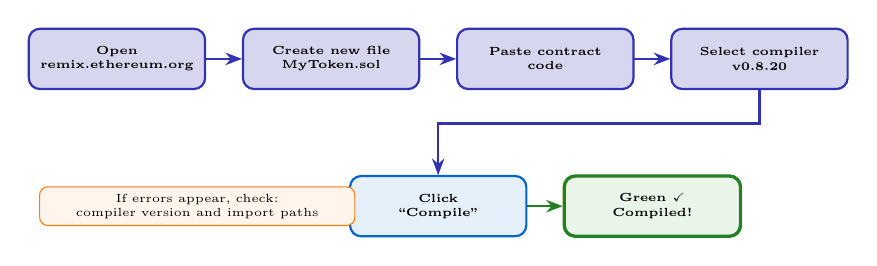
\begin{tikzpicture}[scale=0.85, every node/.style={transform shape},
  stepbox/.style={draw=mlpurple, thick, fill=mllavender4, rounded corners=4pt,
    minimum height=0.9cm, text width=2.4cm, align=center, font=\tiny\bfseries}]

\node[stepbox] (s1) at (0,0) {Open\\remix.ethereum.org};
\node[stepbox] (s2) at (3.2,0) {Create new file\\MyToken.sol};
\node[stepbox] (s3) at (6.4,0) {Paste contract\\code};
\node[stepbox] (s4) at (9.6,0) {Select compiler\\v0.8.20};

\draw[-{Stealth[length=6pt]}, mlpurple, thick] (s1.east) -- (s2.west);
\draw[-{Stealth[length=6pt]}, mlpurple, thick] (s2.east) -- (s3.west);
\draw[-{Stealth[length=6pt]}, mlpurple, thick] (s3.east) -- (s4.west);

\node[stepbox, draw=mlblue, fill=mlblue!10] (s5) at (4.8,-2.2) {Click\\``Compile''};
\node[draw=mlgreen!80!black, very thick, fill=mlgreen!10, rounded corners=4pt,
  minimum height=0.9cm, text width=2.4cm, align=center, font=\tiny\bfseries]
  (s6) at (8.0,-2.2) {Green $\checkmark$\\Compiled!};

\draw[-{Stealth[length=6pt]}, mlpurple, thick] (s4.south) -- ++(0,-0.5) -| (s5.north);
\draw[-{Stealth[length=6pt]}, mlgreen!80!black, thick] (s5.east) -- (s6.west);

% Helpful annotation
\node[draw=mlorange, fill=mlorange!8, rounded corners=3pt, font=\tiny,
      inner sep=3pt, text width=4.5cm, align=center]
      at (1.2,-2.2) {If errors appear, check:\\compiler version and import paths};

\end{tikzpicture}%
}%
\end{center}

\bottomnote{Remix compiles Solidity in your browser --- no installation needed. A green checkmark means success.}
\end{frame}

%% ============================================================
%% FRAME 6: STEP 3 - CONNECT METAMASK
%% ============================================================
\begin{frame}{Step 3 --- Connect MetaMask}
\begin{center}
\adjustbox{max width=\textwidth}{%
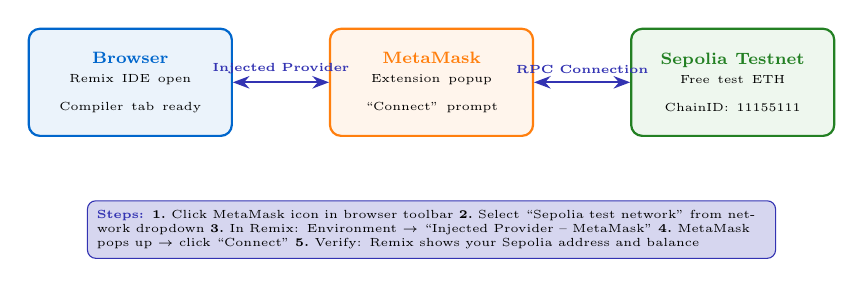
\begin{tikzpicture}[scale=0.85, every node/.style={transform shape},
  bigbox/.style={draw=mlpurple, thick, fill=mllavender4, rounded corners=4pt,
    minimum height=1.6cm, text width=2.8cm, align=center}]

% Browser
\node[bigbox, draw=mlblue, fill=mlblue!8] (browser) at (-4.5,0) {%
  \textbf{\scriptsize\color{mlblue}Browser}\\[2pt]
  \tiny Remix IDE open\\
  \tiny Compiler tab ready};

% MetaMask
\node[bigbox, draw=mlorange, fill=mlorange!8] (meta) at (0,0) {%
  \textbf{\scriptsize\color{mlorange}MetaMask}\\[2pt]
  \tiny Extension popup\\
  \tiny ``Connect'' prompt};

% Sepolia
\node[bigbox, draw=mlgreen!80!black, fill=mlgreen!8] (sepolia) at (4.5,0) {%
  \textbf{\scriptsize\color{mlgreen!80!black}Sepolia Testnet}\\[2pt]
  \tiny Free test ETH\\
  \tiny ChainID: 11155111};

% Arrows
\draw[{Stealth[length=6pt]}-{Stealth[length=6pt]}, mlpurple, thick]
  (browser.east) -- (meta.west)
  node[midway, above, font=\tiny\bfseries] {Injected Provider};

\draw[{Stealth[length=6pt]}-{Stealth[length=6pt]}, mlpurple, thick]
  (meta.east) -- (sepolia.west)
  node[midway, above, font=\tiny\bfseries] {RPC Connection};

% Steps below
\node[draw=mlpurple, fill=mllavender4, rounded corners=3pt, font=\tiny,
      inner sep=4pt, text width=10cm, align=left]
      at (0,-2.2) {%
      \textbf{\color{mlpurple}Steps:}
      \textbf{1.}~Click MetaMask icon in browser toolbar
      \textbf{2.}~Select ``Sepolia test network'' from network dropdown
      \textbf{3.}~In Remix: Environment $\rightarrow$ ``Injected Provider -- MetaMask''
      \textbf{4.}~MetaMask pops up $\rightarrow$ click ``Connect''
      \textbf{5.}~Verify: Remix shows your Sepolia address and balance};

\end{tikzpicture}%
}%
\end{center}

\bottomnote{MetaMask bridges your browser to the blockchain --- Remix talks to Sepolia through it.}
\end{frame}

%% ============================================================
%% FRAME 7: STEP 4 - DEPLOY!
%% ============================================================
\begin{frame}{Step 4 --- Deploy!}
\begin{center}
\adjustbox{max width=\textwidth}{%
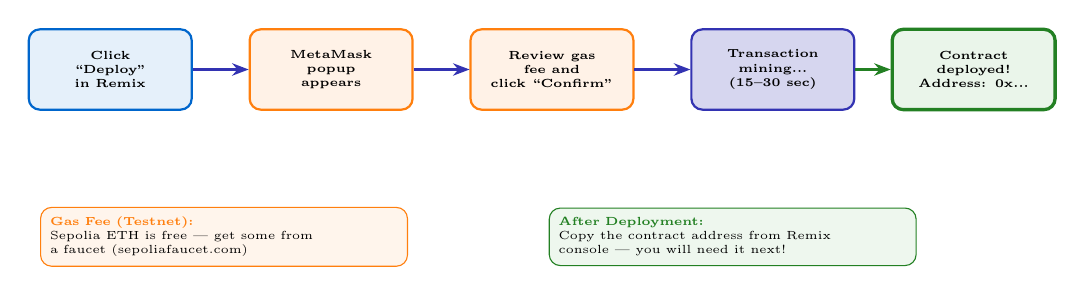
\begin{tikzpicture}[scale=0.85, every node/.style={transform shape},
  stepbox/.style={draw=mlpurple, thick, fill=mllavender4, rounded corners=4pt,
    minimum height=1.2cm, text width=2.2cm, align=center, font=\tiny\bfseries}]

% Main flow
\node[stepbox, draw=mlblue, fill=mlblue!10] (d1) at (-5.5,0.5) {Click\\``Deploy''\\in Remix};

\node[stepbox, draw=mlorange, fill=mlorange!10] (d2) at (-2.2,0.5) {MetaMask\\popup\\appears};

\node[stepbox, draw=mlorange, fill=mlorange!10] (d3) at (1.1,0.5) {Review gas\\fee and\\click ``Confirm''};

\node[stepbox, draw=mlpurple, fill=mllavender4] (d4) at (4.4,0.5) {Transaction\\mining...\\(15--30 sec)};

\node[draw=mlgreen!80!black, very thick, fill=mlgreen!10, rounded corners=4pt,
  minimum height=1.2cm, text width=2.2cm, align=center, font=\tiny\bfseries]
  (d5) at (7.4,0.5) {Contract\\deployed!\\Address: 0x...};

\draw[-{Stealth[length=6pt]}, mlpurple, thick] (d1.east) -- (d2.west);
\draw[-{Stealth[length=6pt]}, mlpurple, thick] (d2.east) -- (d3.west);
\draw[-{Stealth[length=6pt]}, mlpurple, thick] (d3.east) -- (d4.west);
\draw[-{Stealth[length=6pt]}, mlgreen!80!black, thick] (d4.east) -- (d5.west);

% Key info below
\node[draw=mlorange, fill=mlorange!8, rounded corners=4pt, font=\tiny,
      inner sep=4pt, text width=5.2cm, align=left]
      at (-3.8,-2.0) {%
      \textbf{\color{mlorange}Gas Fee (Testnet):}\\
      Sepolia ETH is free --- get some from\\
      a faucet (sepoliafaucet.com)};

\node[draw=mlgreen!80!black, fill=mlgreen!8, rounded corners=4pt, font=\tiny,
      inner sep=4pt, text width=5.2cm, align=left]
      at (3.8,-2.0) {%
      \textbf{\color{mlgreen!80!black}After Deployment:}\\
      Copy the contract address from Remix\\
      console --- you will need it next!};

\end{tikzpicture}%
}%
\end{center}

\bottomnote{Deployment sends your compiled bytecode to the blockchain --- MetaMask signs the transaction for you.}
\end{frame}

%% ============================================================
%% FRAME 8: STEP 5 - VERIFY ON ETHERSCAN
%% ============================================================
\begin{frame}{Step 5 --- Verify on Etherscan}
\begin{center}
\adjustbox{max width=\textwidth}{%
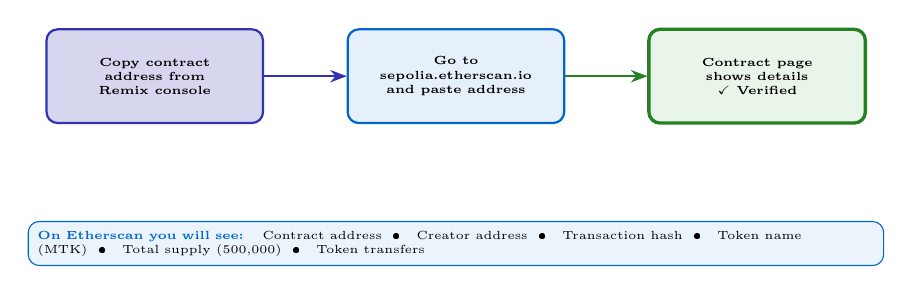
\begin{tikzpicture}[scale=0.85, every node/.style={transform shape},
  stepbox/.style={draw=mlpurple, thick, fill=mllavender4, rounded corners=4pt,
    minimum height=1.4cm, text width=3.0cm, align=center, font=\tiny\bfseries}]

\node[stepbox] (v1) at (-4.5,0.5) {Copy contract\\address from\\Remix console};

\node[stepbox, draw=mlblue, fill=mlblue!10] (v2) at (0,0.5) {Go to\\sepolia.etherscan.io\\and paste address};

\node[draw=mlgreen!80!black, very thick, fill=mlgreen!10, rounded corners=4pt,
  minimum height=1.4cm, text width=3.0cm, align=center, font=\tiny\bfseries]
  (v3) at (4.5,0.5) {Contract page\\shows details\\$\checkmark$ Verified};

\draw[-{Stealth[length=6pt]}, mlpurple, thick] (v1.east) -- (v2.west);
\draw[-{Stealth[length=6pt]}, mlgreen!80!black, thick] (v2.east) -- (v3.west);

% What you see
\node[draw=mlblue, fill=mlblue!8, rounded corners=4pt, font=\tiny,
      inner sep=4pt, text width=12.5cm, align=left]
      at (0,-2.0) {%
      \textbf{\color{mlblue}On Etherscan you will see:}~~
      Contract address~~\textbullet~~
      Creator address~~\textbullet~~
      Transaction hash~~\textbullet~~
      Token name (MTK)~~\textbullet~~
      Total supply (500,000)~~\textbullet~~
      Token transfers};

\end{tikzpicture}%
}%
\end{center}

\bottomnote{Etherscan is the blockchain explorer --- it confirms your contract is live and lets anyone inspect it.}
\end{frame}

%% ============================================================
%% FRAME 9: STEP 6 - ADD TOKEN TO METAMASK
%% ============================================================
\begin{frame}{Step 6 --- Add Token to MetaMask}
\begin{center}
\adjustbox{max width=\textwidth}{%
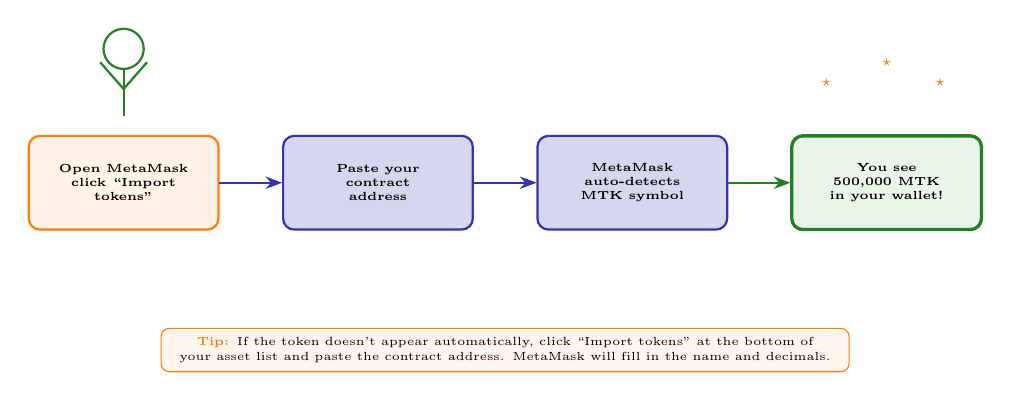
\begin{tikzpicture}[scale=0.85, every node/.style={transform shape},
  stepbox/.style={draw=mlpurple, thick, fill=mllavender4, rounded corners=4pt,
    minimum height=1.4cm, text width=2.6cm, align=center, font=\tiny\bfseries}]

\node[stepbox, draw=mlorange, fill=mlorange!10] (a1) at (-5,0.5) {Open MetaMask\\click ``Import\\tokens''};

\node[stepbox] (a2) at (-1.2,0.5) {Paste your\\contract\\address};

\node[stepbox] (a3) at (2.6,0.5) {MetaMask\\auto-detects\\MTK symbol};

\node[draw=mlgreen!80!black, very thick, fill=mlgreen!10, rounded corners=4pt,
  minimum height=1.4cm, text width=2.6cm, align=center, font=\tiny\bfseries]
  (a4) at (6.4,0.5) {You see\\500,000 MTK\\in your wallet!};

\draw[-{Stealth[length=6pt]}, mlpurple, thick] (a1.east) -- (a2.west);
\draw[-{Stealth[length=6pt]}, mlpurple, thick] (a2.east) -- (a3.west);
\draw[-{Stealth[length=6pt]}, mlgreen!80!black, thick] (a3.east) -- (a4.west);

% Celebration
\node[font=\scriptsize, mlorange] at (5.5,2.0) {$\star$};
\node[font=\scriptsize, mlorange] at (7.2,2.0) {$\star$};
\node[font=\scriptsize, mlorange] at (6.4,2.3) {$\star$};

% Celebrating stick figure
\draw[mlgreen!80!black, thick] (-5,2.5) circle (0.3);
\draw[mlgreen!80!black, thick] (-5,2.2) -- (-5,1.5);
\draw[mlgreen!80!black, thick] (-5,1.9) -- (-5.35,2.3);
\draw[mlgreen!80!black, thick] (-5,1.9) -- (-4.65,2.3);

% Info box
\node[draw=mlorange, fill=mlorange!8, rounded corners=3pt, font=\tiny,
      inner sep=4pt, text width=10cm, align=center]
      at (0.7,-2.0) {%
      \textbf{\color{mlorange}Tip:}
      If the token doesn't appear automatically, click ``Import tokens'' at the bottom of your asset list and paste the contract address. MetaMask will fill in the name and decimals.};

\end{tikzpicture}%
}%
\end{center}

\bottomnote{MetaMask needs to ``know'' about custom tokens --- importing by address links your token to your wallet view.}
\end{frame}

%% ============================================================
%% FRAME 10: THE COMPLETE RECIPE CARD
%% ============================================================
\begin{frame}{The Complete Recipe Card}
\vspace{-2mm}
\begin{center}
\adjustbox{max width=\textwidth}{%
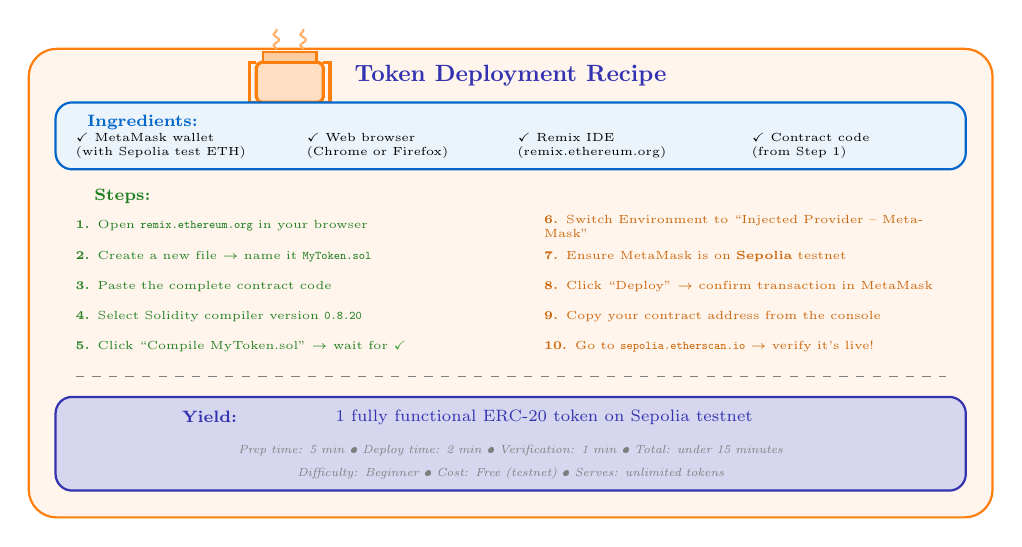
\begin{tikzpicture}[scale=0.85, every node/.style={transform shape}]

% === Recipe Card Background ===
\draw[mlorange, thick, fill=mlorange!8, rounded corners=10pt] (-7.2,-3.2) rectangle (7.2,3.8);

% === Title ===
\node[font=\normalsize\bfseries, mlpurple] at (0,3.4) {Token Deployment Recipe};

% === Pot Icon (left of title) ===
\draw[mlorange, very thick, fill=mlorange!25, rounded corners=2pt] (-3.8,3.0) rectangle (-2.8,3.6);
\draw[mlorange, very thick] (-3.8,3.6) -- (-3.9,3.6) -- (-3.9,3.0) -- (-3.8,3.0);
\draw[mlorange, very thick] (-2.8,3.6) -- (-2.7,3.6) -- (-2.7,3.0) -- (-2.8,3.0);
\draw[mlorange, thick, fill=mlorange!40] (-3.7,3.6) rectangle (-2.9,3.75);
% Steam
\draw[mlorange!60, thick, decorate, decoration={snake, amplitude=1pt, segment length=4pt}]
  (-3.5,3.8) -- (-3.5,4.1);
\draw[mlorange!60, thick, decorate, decoration={snake, amplitude=1pt, segment length=4pt}]
  (-3.1,3.8) -- (-3.1,4.1);

% === Ingredients Box (top, horizontal) ===
\draw[mlblue, thick, fill=mlblue!8, rounded corners=6pt] (-6.8,2.0) rectangle (6.8,3.0);
\node[font=\scriptsize\bfseries, mlblue] at (-5.5,2.7) {Ingredients:};
\node[font=\tiny, text width=3.0cm, align=left] at (-5.0,2.35)
     {$\checkmark$ MetaMask wallet\\(with Sepolia test ETH)};
\node[font=\tiny, text width=2.5cm, align=left] at (-1.8,2.35)
     {$\checkmark$ Web browser\\(Chrome or Firefox)};
\node[font=\tiny, text width=2.8cm, align=left] at (1.5,2.35)
     {$\checkmark$ Remix IDE\\(remix.ethereum.org)};
\node[font=\tiny, text width=2.8cm, align=left] at (5.0,2.35)
     {$\checkmark$ Contract code\\(from Step 1)};

% === Steps (single column, numbered) ===
\node[font=\scriptsize\bfseries, mlgreen!80!black] at (-5.8,1.6) {Steps:};

% Left column (steps 1-5)
\node[font=\tiny, mlgreen!80!black, text width=6.0cm, align=left] at (-3.5,1.15) {%
\textbf{1.} Open \texttt{remix.ethereum.org} in your browser};
\node[font=\tiny, mlgreen!80!black, text width=6.0cm, align=left] at (-3.5,0.7) {%
\textbf{2.} Create a new file $\rightarrow$ name it \texttt{MyToken.sol}};
\node[font=\tiny, mlgreen!80!black, text width=6.0cm, align=left] at (-3.5,0.25) {%
\textbf{3.} Paste the complete contract code};
\node[font=\tiny, mlgreen!80!black, text width=6.0cm, align=left] at (-3.5,-0.2) {%
\textbf{4.} Select Solidity compiler version \texttt{0.8.20}};
\node[font=\tiny, mlgreen!80!black, text width=6.0cm, align=left] at (-3.5,-0.65) {%
\textbf{5.} Click ``Compile MyToken.sol'' $\rightarrow$ wait for \textcolor{mlgreen}{$\checkmark$}};

% Right column (steps 6-10)
\node[font=\tiny, mlorange!80!black, text width=6.0cm, align=left] at (3.5,1.15) {%
\textbf{6.} Switch Environment to ``Injected Provider -- MetaMask''};
\node[font=\tiny, mlorange!80!black, text width=6.0cm, align=left] at (3.5,0.7) {%
\textbf{7.} Ensure MetaMask is on \textbf{Sepolia} testnet};
\node[font=\tiny, mlorange!80!black, text width=6.0cm, align=left] at (3.5,0.25) {%
\textbf{8.} Click ``Deploy'' $\rightarrow$ confirm transaction in MetaMask};
\node[font=\tiny, mlorange!80!black, text width=6.0cm, align=left] at (3.5,-0.2) {%
\textbf{9.} Copy your contract address from the console};
\node[font=\tiny, mlorange!80!black, text width=6.0cm, align=left] at (3.5,-0.65) {%
\textbf{10.} Go to \texttt{sepolia.etherscan.io} $\rightarrow$ verify it's live!};

% === Divider line between steps and yield ===
\draw[mlgray, thin, dashed] (-6.5,-1.1) -- (6.5,-1.1);

% === Yield / Result Box ===
\draw[mlpurple, thick, fill=mllavender4, rounded corners=6pt] (-6.8,-2.8) rectangle (6.8,-1.4);
\node[font=\scriptsize\bfseries, mlpurple] at (-4.5,-1.7) {Yield:};
\node[font=\scriptsize, mlpurple] at (0.5,-1.7)
     {1 fully functional ERC-20 token on Sepolia testnet};
\node[font=\tiny\itshape, mlgray, text width=12cm, align=center] at (0,-2.2)
     {Prep time: 5 min \textbullet\ Deploy time: 2 min \textbullet\ Verification: 1 min \textbullet\ Total: under 15 minutes};
\node[font=\tiny\itshape, mlgray, text width=12cm, align=center] at (0,-2.55)
     {Difficulty: Beginner \textbullet\ Cost: Free (testnet) \textbullet\ Serves: unlimited tokens};

\end{tikzpicture}%
}%
\end{center}

\bottomnote{Follow this recipe step by step --- you will have your own token deployed in under 15 minutes.}
\end{frame}

%% ============================================================
%% FRAME 11: WHAT CAN GO WRONG? (Troubleshooting)
%% ============================================================
\begin{frame}{What Can Go Wrong?}
\vspace{-1mm}
\begin{center}
\adjustbox{max width=\textwidth, max totalheight=6.5cm}{%
\begin{tabular}{>{\raggedright\arraybackslash}p{5.5cm} >{\raggedright\arraybackslash}p{6.5cm}}
\toprule
\textbf{\color{mlred}Common Error} & \textbf{\color{mlgreen!80!black}Fix} \\
\midrule
\textcolor{mlred}{Compiler version mismatch}
& Select \texttt{0.8.20} in Remix compiler dropdown \\[3pt]
\textcolor{mlred}{``ParserError: Source not found''}
& Remix auto-imports OpenZeppelin --- ensure you are online \\[3pt]
\textcolor{mlred}{MetaMask not connecting}
& Refresh page, then Environment $\rightarrow$ ``Injected Provider'' \\[3pt]
\textcolor{mlred}{``Insufficient funds for gas''}
& Get free Sepolia ETH from \texttt{sepoliafaucet.com} \\[3pt]
\textcolor{mlred}{Transaction stuck / pending}
& Speed up in MetaMask or wait --- Sepolia can be slow \\[3pt]
\textcolor{mlred}{Wrong network (Mainnet!)}
& \textbf{STOP} --- switch to Sepolia immediately. Mainnet costs real money \\[3pt]
\textcolor{mlred}{Token not visible in wallet}
& Import token manually: paste contract address in MetaMask \\[3pt]
\textcolor{mlred}{``Exceeds cap'' on mint}
& You hit MAX\_SUPPLY (1M). Burn tokens first or adjust cap \\
\bottomrule
\end{tabular}%
}%
\end{center}

\bottomnote{Most errors come from wrong network or compiler version --- always double-check these two settings first.}
\end{frame}

%% ============================================================
%% FRAME 12: KEY TAKEAWAYS
%% ============================================================
\begin{frame}{Key Takeaways}
\vspace{-1mm}
\begin{center}
\adjustbox{max width=\textwidth}{%
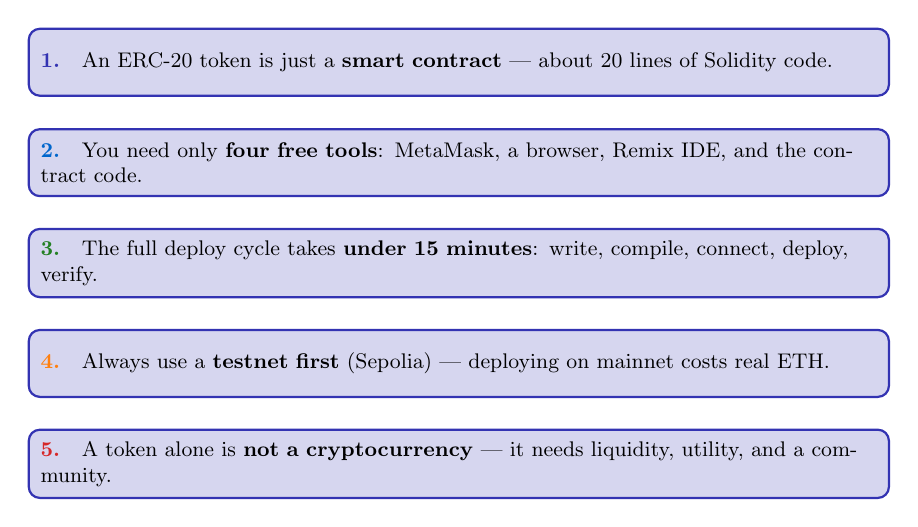
\begin{tikzpicture}[scale=0.85, every node/.style={transform shape},
  takebox/.style={draw=mlpurple, thick, fill=mllavender4, rounded corners=4pt,
    minimum height=1.0cm, text width=12.5cm, align=left, inner sep=5pt, font=\small}]

\node[takebox] (t1) at (0,3.0) {%
  \textbf{\color{mlpurple}1.}\quad
  An ERC-20 token is just a \textbf{smart contract} --- about 20 lines of Solidity code.};

\node[takebox] (t2) at (0,1.5) {%
  \textbf{\color{mlblue}2.}\quad
  You need only \textbf{four free tools}: MetaMask, a browser, Remix IDE, and the contract code.};

\node[takebox] (t3) at (0,0.0) {%
  \textbf{\color{mlgreen!80!black}3.}\quad
  The full deploy cycle takes \textbf{under 15 minutes}: write, compile, connect, deploy, verify.};

\node[takebox] (t4) at (0,-1.5) {%
  \textbf{\color{mlorange}4.}\quad
  Always use a \textbf{testnet first} (Sepolia) --- deploying on mainnet costs real ETH.};

\node[takebox] (t5) at (0,-3.0) {%
  \textbf{\color{mlred}5.}\quad
  A token alone is \textbf{not a cryptocurrency} --- it needs liquidity, utility, and a community.};

\end{tikzpicture}%
}%
\end{center}

\bottomnote{Creating a token is the easy part --- making it valuable requires real-world adoption and utility.}
\end{frame}

\end{document}
